% ============================================================================
% main.tex -- Template di tesi in LaTeX (pdfLaTeX + biber), PDF/A-1b opzionale
%
% I DATI DELLA TESI (titolo, relatore, candidato, ...) E GLI INTERRUTTORI
% SI MODIFICANO IN config.tex, NON QUI.
%
% Compilazione consigliata:   latexmk main.tex    (vedi README.md)
% Con PDF/A attivo serve anche il file main.xmpdata (stesso nome di questo
% file, estensione .xmpdata).
% Il nome del file principale non deve avere spazi, accenti o caratteri speciali.
% ============================================================================

% Dati e interruttori della tesi (frontespizio, metadati, PDF/A, epigrafe)
% ============================================================================
% config.tex  --  QUI SI MODIFICANO I DATI DELLA TESI
% ============================================================================
% Compila questo file per primo: frontespizio, metadati del PDF (main.xmpdata)
% e interruttori leggono tutto da qui. Non servono modifiche al frontespizio.
%
% ATTENZIONE: nei valori evita comandi LaTeX complessi (soprattutto in
% \TitoloTesi e \Candidato, che finiscono anche nei metadati del PDF).
% Le lettere accentate e l'apostrofo vanno bene; per le virgolette usa ' e ".
% ============================================================================

% ----------------------------------------------------------------------------
% Dati del frontespizio e dei metadati del PDF
% ----------------------------------------------------------------------------
\newcommand{\TitoloTesi}{Titolo della tesi: sottotitolo se presente}
\newcommand{\TipoTesi}{Tesi sperimentale di specializzazione}
\newcommand{\TipoCorso}{Scuola di Specializzazione in}
\newcommand{\NomeCorso}{Nome della Scuola di Specializzazione}
\newcommand{\Dipartimento}{Dipartimento di Nome del Dipartimento}

\newcommand{\Relatore}{Prof. Nome Cognome}
% Correlatore: lascia vuoto (\newcommand{\Correlatore}{}) se non c'e'.
\newcommand{\Correlatore}{}
\newcommand{\Candidato}{Dott. Nome Cognome}
\newcommand{\Matricola}{XX0000000}
\newcommand{\AnnoAccademico}{AAAA/AAAA}

% Metadati PDF aggiuntivi (usati da main.xmpdata). Le parole chiave si
% separano con \sep, come nell'esempio.
\newcommand{\ParoleChiaveTesi}{Parola chiave 1\sep Parola chiave 2\sep Parola chiave 3}

% Logo dell'Ateneo (vedi FIGURE/README.md). Per rimuoverlo dal frontespizio
% basta lasciare vuoto il valore: \newcommand{\FileLogo}{}
% ATTENZIONE PDF/A: il file deve essere PNG/JPG/PDF senza canale alpha.
\newcommand{\FileLogo}{FIGURE/logo_unicampania.png}

% ----------------------------------------------------------------------------
% Interruttori (\...true attiva, \...false disattiva)
% ----------------------------------------------------------------------------
% PDF/A-1b: formato per l'archiviazione a lungo termine, richiesto da alcune
% biblioteche d'Ateneo. VERIFICA con la tua biblioteca se serve davvero.
% Se lo disattivi, main.xmpdata viene ignorato e si usa un PDF normale.
\newif\ifpdfa
\pdfatrue

% Pagine facoltative. Metti \...false per toglierle dal PDF.
% Il testo si scrive nei rispettivi file.

% Epigrafe: pagina di citazioni dopo il frontespizio (epigrafe.tex).
\newif\ifepigrafe
\epigrafetrue

% Dedica: pagina con una dedica, dopo l'epigrafe (dedica.tex).
\newif\ifdedica
\dedicatrue

% Ringraziamenti: in fondo alla tesi, dopo la bibliografia (ringraziamenti.tex).
\newif\ifringraziamenti
\ringraziamentitrue

% Elenco delle abbreviazioni: dopo l'indice e gli elenchi di figure e tabelle
% (abbreviazioni.tex).
\newif\ifabbreviazioni
\abbreviazionitrue


% PDF/A-1 richiede al massimo la versione PDF 1.4: senza questa riga il PDF esce
% in 1.7 pur dichiarando PDF/A-1b nei metadati. Deve stare PRIMA di \documentclass.
\ifpdfa\pdfminorversion=4 \fi

\documentclass[
  a4paper,
  oneside,        % Stampa solo fronte
  open=right,     % I capitoli iniziano su qualsiasi pagina (niente pagine bianche)
  fontsize=12pt   % Dimensione carattere
]{scrreprt}

% ----------------------------------------------------------------------------
% Codifica dei font
% ----------------------------------------------------------------------------
% T1 gestisce bene gli accentati; textcomp serve per \texteuro (il simbolo €
% digitato direttamente puo' non comparire con pdfLaTeX: usa \texteuro{}).
\usepackage[T1]{fontenc}
\usepackage{textcomp}

\usepackage{setspace}
\onehalfspacing

\addtokomafont{disposition}{\rmfamily} % titoli con lo stesso font del testo

% Margini (modificali in base alle indicazioni)
\usepackage[
  left=3cm,
  right=2cm,
  top=3.5cm,
  bottom=3.5cm,
  footskip=1cm
]{geometry}

% ----------------------------------------------------------------------------
% PDF/A-1b e hyperref
% ----------------------------------------------------------------------------
% pdfx carica internamente hyperref e legge i metadati da main.xmpdata
% (che a sua volta legge i valori da config.tex).
% Se in config.tex hai impostato \pdfafalse, si usa hyperref "normale".
\ifpdfa
  \usepackage[a-1b]{pdfx}
\else
  \usepackage{hyperref}
  \providecommand{\sep}{, }
  \hypersetup{
    pdftitle    = {\TitoloTesi},
    pdfauthor   = {\Candidato},
    pdfkeywords = {\ParoleChiaveTesi},
    pdflang     = {it-IT}
  }
\fi

\hypersetup{
  bookmarksnumbered   = true,        % Segnalibri con numeri dei capitoli/sezioni
  bookmarksopen       = true,        % Albero dei segnalibri aperto
  bookmarksopenlevel  = 0,           % Inizialmente solo i capitoli
  bookmarksdepth      = 3,           % Segnalibri fino alle sottosezioni
  pdfpagemode         = UseOutlines, % Barra laterale dei segnalibri all'apertura
  pdfstartview        = Fit,
  plainpages          = false,       % Evita conflitti tra numerazione romana e araba
  colorlinks          = true,        % Link come testo colorato, non riquadri
  linkcolor           = black,
  citecolor           = black,
  urlcolor            = black,
  filecolor           = black
}

% ----------------------------------------------------------------------------
% Lingua
% ----------------------------------------------------------------------------
% Deve corrispondere a \Language in main.xmpdata. L'inglese e' la lingua
% secondaria (utile per l'abstract in inglese, se richiesto, o per terminologia
% nel testo).
\usepackage[english, main=italian]{babel}

% ----------------------------------------------------------------------------
% Tipografia, grafica, tabelle
% ----------------------------------------------------------------------------
\usepackage{microtype}
\usepackage{amsmath}
\usepackage{graphicx}
\usepackage{multirow}
\usepackage{tabularx}
\usepackage{float}
\usepackage{adjustbox}
\usepackage{longtable}
\usepackage{booktabs}
\usepackage{array}
\usepackage{pdflscape}
\usepackage{pdfpages}   % per includere PDF esterni (es. dichiarazioni firmate)
\usepackage{caption}
\usepackage{indentfirst}

% ----------------------------------------------------------------------------
% Piè di pagina con numero di pagina
% ----------------------------------------------------------------------------
\usepackage[automark, headsepline=false, footsepline=false]{scrlayer-scrpage}

% Testo al centro del piè di pagina (es. \renewcommand{\currentreprint}{Bozza})
\newcommand{\currentreprint}{}

\defpairofpagestyles{reprint}{%
  \clearpairofpagestyles
  \ofoot*{\pagemark}                    % Numero di pagina a destra
  \cfoot*{\footnotesize\currentreprint} % Testo opzionale al centro
}

% ----------------------------------------------------------------------------
% Riferimenti incrociati intelligenti
% ----------------------------------------------------------------------------
% Scrivi \cref{fig:esempio} e LaTeX produce "Figura 1.1" da solo.
\usepackage{cleveref}

\crefname{table}{Tabella}{Tabelle}
\Crefname{table}{Tabella}{Tabelle}
\crefname{figure}{Figura}{Figure}
\Crefname{figure}{Figura}{Figure}
\crefname{appendix}{Appendice}{Appendici}
\Crefname{appendix}{Appendice}{Appendici}
\crefname{chapter}{Capitolo}{Capitoli}
\Crefname{chapter}{Capitolo}{Capitoli}
\crefname{section}{Sezione}{Sezioni}
\Crefname{section}{Sezione}{Sezioni}
\crefname{subsection}{Sezione}{Sezioni}
\Crefname{subsection}{Sezione}{Sezioni}
\crefname{subsubsection}{Sezione}{Sezioni}
\Crefname{subsubsection}{Sezione}{Sezioni}
\crefname{equation}{equazione}{equazioni}
\Crefname{equation}{Equazione}{Equazioni}

% ----------------------------------------------------------------------------
% Bibliografia (biblatex + biber)
% ----------------------------------------------------------------------------
% csquotes evita avvisi di biblatex; style=english per virgolette alla inglese
% (con main=italian altrimenti userebbe le virgolette basse).
\usepackage[style=english]{csquotes}

\usepackage[
    backend=biber,
    hyperref=true,
    style=numeric-comp,   % citazioni numeriche [1-3]; per autore-anno: style=authoryear
    sorting=none,         % numerazione in ordine di prima citazione
    maxbibnames=10,
    minbibnames=3,
    giveninits=true,
    isbn=false,
    doi=true,
    url=true,
    eprint=false
]{biblatex}

% L'URL si stampa solo per le voci di tipo @online
\AtEveryBibitem{%
  \ifentrytype{online}{}{%
    \clearfield{url}%
    \clearfield{urldate}%
  }%
}

% Titoli degli articoli senza virgolette
\DeclareFieldFormat[article,inbook,incollection,inproceedings,patent,thesis,unpublished]{title}{#1}

\addbibresource{bibliografia.bib}

% ----------------------------------------------------------------------------
% Epigrafe (pagina di citazioni): attivabile da config.tex con \epigrafetrue
% ----------------------------------------------------------------------------
\usepackage{epigraph}
\setlength{\epigraphwidth}{0.75\textwidth}
\renewcommand{\textflush}{flushright} % testo allineato a destra
\setlength{\epigraphrule}{0pt}        % nessuna riga tra testo e fonte

% ----------------------------------------------------------------------------
% Compilare solo alcuni capitoli (\includeonly)
%
% A cosa serve: mentre scrivi, compili solo i capitoli su cui stai lavorando.
% La compilazione e' piu' veloce e i riferimenti agli altri capitoli
% (numeri di pagina, figure, tabelle, sezioni) restano corretti.
%
% Come si usa:
%   1. Compila prima l'intera tesi, una volta. Cosi' LaTeX crea i file .aux
%      di tutti i capitoli, che servono a ricordare i loro numeri.
%   2. Togli il % davanti a \includeonly qui sotto e lascia nella lista
%      solo i capitoli che vuoi compilare (puoi anche lasciarne piu' di uno).
%   3. Ricompila con "latexmk main.tex".
%   4. PRIMA DELLA VERSIONE FINALE rimetti il % davanti a \includeonly
%      (oppure elenca di nuovo tutti i capitoli). Se lo dimentichi, il PDF
%      che consegni conterra' solo i capitoli elencati.
%
% Attenzione:
%   - Scrivi i nomi esattamente come in \include, senza ".tex"
%     (es. BODY/1_esempio). Se un nome e' sbagliato, quel capitolo viene
%     saltato senza alcun errore.
%   - Funziona solo con i capitoli caricati con \include, non con \input.
%     Frontespizio e abstract usano \input, quindi vengono sempre composti.
% ----------------------------------------------------------------------------
%\includeonly{
%  BODY/1_esempio,
%  BODY/appendice
%}

\begin{document}
\pagestyle{reprint}
% Frontespizio, epigrafe e dedica (senza numero visibile) usano numerazione a lettere:
% serve a dare ad hyperref destinazioni uniche (altrimenti "page.1" e "page.2"
% verrebbero ripetute quando la numerazione riparte da capo).
\pagenumbering{alph}

% ---- Frontmatter ----
% ----------------------------------------------------------------------------
% frontespizio.tex
% Non serve modificarlo: legge tutti i dati da config.tex.
% NOTA: l'intestazione e il layout sono un esempio, non un modello ufficiale
% dell'Ateneo. Controlla sempre le indicazioni della tua Scuola/Segreteria.
% ----------------------------------------------------------------------------
\begin{titlepage}
    \centering

    % --- INTESTAZIONE ---
    {\Large \textbf{UNIVERSITÀ DEGLI STUDI DELLA CAMPANIA}} \\
    \vspace{0.2cm}
    {\Large \textbf{``LUIGI VANVITELLI''}} \\

    \vspace{1.2cm}

    % --- LOGO ---
    \ifx\FileLogo\empty\else
      \includegraphics[width=0.50\textwidth]{\FileLogo} \\
    \fi

    \vspace{2cm}

    % --- SCUOLA/CORSO E DIPARTIMENTO ---
    {\Large \TipoCorso} \\
    {\Large \textbf{\NomeCorso}} \\

    \vspace{0.5cm}

    {\Large \Dipartimento} \\

    \vspace{2cm}

    % --- TITOLO ---
    {\Large \MakeUppercase{\TipoTesi}} \\
    \vspace{1cm}
    {\Large \textbf{\TitoloTesi}} \\

    \vfill % Spinge il blocco successivo verso il fondo pagina

    % --- RELATORE E CANDIDATO ---
    \begin{minipage}[t]{0.45\textwidth}
        \begin{flushleft} \large
            \emph{Relatore:}\\
            \Relatore
            \ifx\Correlatore\empty\else
              \\[0.8em]
              \emph{Correlatore:}\\
              \Correlatore
            \fi
        \end{flushleft}
    \end{minipage}
    \hfill
    \begin{minipage}[t]{0.45\textwidth}
        \begin{flushright} \large
            \emph{Candidato:} \\
            \Candidato \\
            Matr. \Matricola
        \end{flushright}
    \end{minipage}

    \vspace{1.5cm}

    % --- ANNO ACCADEMICO ---
    {\large Anno Accademico \AnnoAccademico}

\end{titlepage}


\ifepigrafe
  % ----------------------------------------------------------------------------
% epigrafe.tex
% Pagina di citazioni in apertura della tesi (dopo il frontespizio).
% Per non usarla: in config.tex metti \epigrafefalse.
% Per aggiungere altre citazioni ripeti \epigraph{testo}{fonte}: l'ordine
% in cui compaiono e' l'ordine di impaginazione.
% Prima di usare una citazione verifica sempre testo e fonte originali.
% ----------------------------------------------------------------------------
\thispagestyle{empty}
\vspace*{\fill}

\epigraph{\itshape Do. Or do not. There is no try.}%
{--- Yoda, \textit{The Empire Strikes Back} (1980)}

\vspace*{\fill}
\newpage

\fi

\ifdedica
  % ----------------------------------------------------------------------------
% dedica.tex
% Pagina di dedica, dopo l'epigrafe e prima del riassunto.
% Per non usarla: in config.tex metti \dedicafalse.
% ----------------------------------------------------------------------------
\thispagestyle{empty}
\vspace*{\fill}

\begin{flushright}
  \itshape
  Dedica della tesi.\\
  A chi vuoi tu.
\end{flushright}

\vspace*{\fill}
\newpage

\fi

\pagenumbering{roman}
\setcounter{page}{1}

% ----------------------------------------------------------------------------
% abstract.tex -- riassunto in italiano
% e abstract in inglese (opzionale, da sbloccare)
% L'asterisco (\chapter*) evita la numerazione come capitolo normale.
% Se serve solo una delle due versioni, cancella l'altra.
% ----------------------------------------------------------------------------
\chapter*{Abstract}
Questo \`e l'abstract della tesi in italiano. Spiega brevemente il problema affrontato,
gli obiettivi, i materiali e i metodi, i risultati principali e le conclusioni.

% \clearpage

% \begin{otherlanguage}{english}
% \chapter*{Abstract}
% This is the English abstract. Briefly describe the background, objectives, methods,
% main results and conclusions of the thesis.
% \end{otherlanguage}

\tableofcontents
\listoffigures
\listoftables

\ifabbreviazioni
  % ----------------------------------------------------------------------------
% abbreviazioni.tex
% Elenco delle abbreviazioni, dopo l'indice e gli elenchi di figure e tabelle.
% Per non usarlo: in config.tex metti \abbreviazionifalse.
% Aggiungi una riga per ogni abbreviazione, in ordine alfabetico:
%   SIGLA & Significato \\
% ----------------------------------------------------------------------------
\chapter*{Elenco delle abbreviazioni}

\begin{longtable}{@{}p{3cm}p{\dimexpr\linewidth-3cm\relax}@{}}
  ADR   & Adverse Drug Reaction (reazione avversa a farmaco) \\
  AIFA  & Agenzia Italiana del Farmaco \\
  EMA   & European Medicines Agency \\
\end{longtable}

\fi

\clearpage

% ---- Main matter: numeri arabi ----
\pagenumbering{arabic}
\setcounter{page}{1}

% Capitoli con \include (non \input) per poter usare \includeonly.
% Per aggiungere un capitolo: crea BODY/2_nome.tex e aggiungi qui sotto
% \include{BODY/2_nome} (senza .tex).
% ----------------------------------------------------------------------------
% BODY/1_esempio.tex -- capitolo di esempio
% Mostra gli elementi piu' comuni: sezioni, citazioni, formule, figure,
% tabelle e riferimenti incrociati. Sostituiscilo con il tuo primo capitolo.
% Convenzione consigliata: un file per capitolo (BODY/2_nome.tex, ...), poi
% aggiungi \include{BODY/2_nome} in main.tex.
% ----------------------------------------------------------------------------
\chapter{Capitolo di esempio}
\label{cap:esempio}

\section{Citazioni e bibliografia}
\label{sec:citazioni}

Le citazioni numeriche si inseriscono con \verb|\cite{chiave}|, dove la chiave
\`e quella definita in \texttt{bibliografia.bib}. Un singolo riferimento appare
come~\cite{wilkinson_fair_2016}; pi\`u riferimenti vengono compattati
automaticamente~\cite{lamport_latex_1994,knuth_texbook_1984}. Anche le risorse
web possono essere citate~\cite{ctan_biblatex}.

\section{Formule}
\label{sec:formule}

Una formula in linea si scrive tra dollari, ad esempio $\bar{x} = \frac{1}{n}\sum_{i=1}^{n} x_i$.
Una formula numerata e richiamabile con \verb|\cref| usa l'ambiente \texttt{equation}:
\begin{equation}
  \mathrm{OR} = \frac{a \cdot d}{b \cdot c}
  \label{eq:odds_ratio}
\end{equation}
come mostra l'\cref{eq:odds_ratio}.

\section{Figure}
\label{sec:figure}

La \cref{fig:esempio} mostra una figura con didascalia e riferimento incrociato:
\`e un esempio di \emph{correlazione spuria}, due serie che si muovono insieme
($r = 0.67$) senza alcun legame causale~\cite{vigen_spurious_2024}. In PDF/A-1b usa
immagini \textbf{senza canale alpha}: vedi il \texttt{README.md}.

\begin{figure}[htbp]
  \centering
  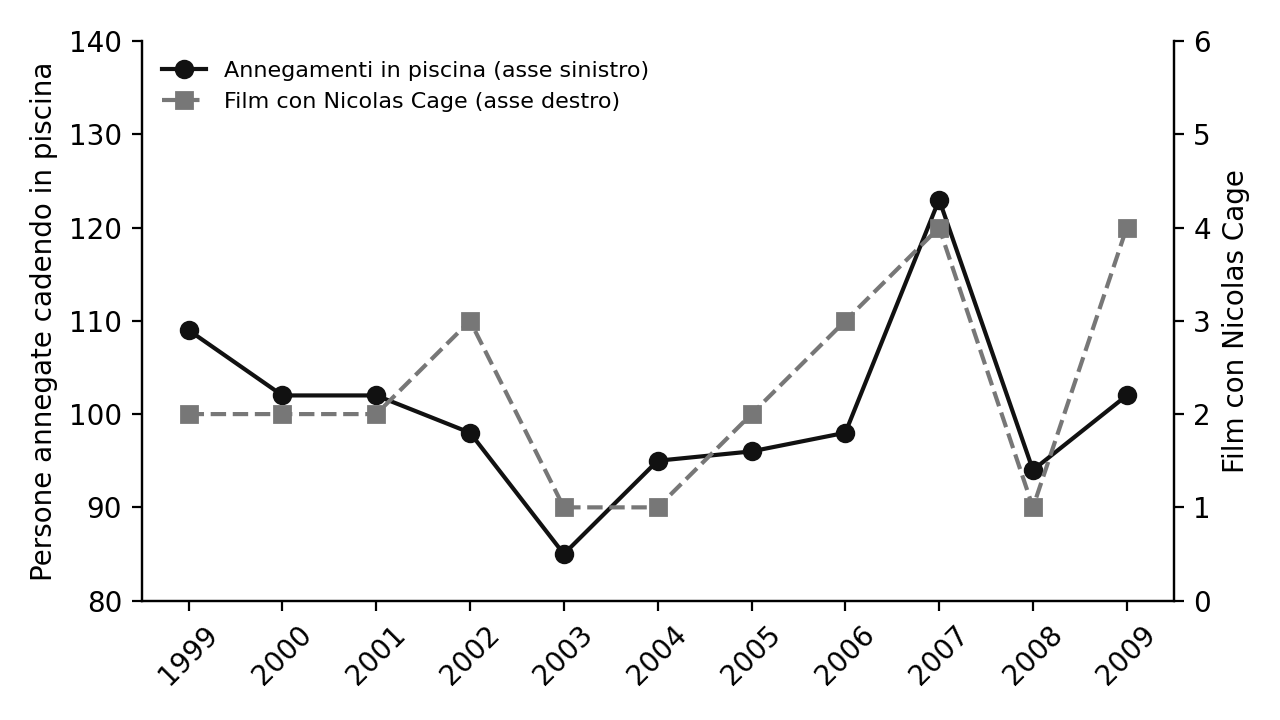
\includegraphics[width=0.8\textwidth]{FIGURE/correlazione_spuria.png}
  \caption{Persone annegate cadendo in piscina e film con Nicolas Cage, 1999--2009
  (correlazione spuria) \cite{vigen_spurious_2024}}
  \label{fig:esempio}
\end{figure}

\section{Tabelle}
\label{sec:tabelle}

La \cref{tab:esempio} usa il pacchetto \texttt{booktabs}, che produce tabelle
pulite con linee orizzontali ben spaziate e senza linee verticali.

\begin{table}[htbp]
  \centering
  \caption{Esempio di tabella (dati fittizi).}
  \label{tab:esempio}
  \begin{tabular}{lrr}
    \toprule
    Gruppo & Soggetti (n) & Eventi (\%) \\
    \midrule
    Gruppo A & 120 & 12.5 \\
    Gruppo B & 118 & 8.5 \\
    \bottomrule
  \end{tabular}
\end{table}

Per i riferimenti interni usa \verb|\label| e \verb|\cref|: vedi l'\cref{app:esempio}
e la \cref{sec:citazioni}.


\appendix
% Da qui i capitoli diventano "Appendice A", "Appendice B", ecc.
% Fa si' che \cref scriva "Appendice A" (e non "Capitolo A") per questi capitoli.
\crefalias{chapter}{appendix}
% ----------------------------------------------------------------------------
% BODY/appendice.tex -- appendice di esempio
% Dopo \appendix in main.tex i capitoli diventano "Appendice A", "B", ...
% ----------------------------------------------------------------------------
\chapter{Materiale supplementare}
\label{app:esempio}

\section{Tabella supplementare}

La \cref{tab:supp_esempio} mostra una tabella supplementare di esempio.

\begin{table}[htbp]
  \centering
  \caption{Esempio di tabella supplementare (dati fittizi).}
  \label{tab:supp_esempio}
  \begin{tabular}{lll}
    \toprule
    Variabile & Descrizione & Esempio \\
    \midrule
    Anno & Anno di pubblicazione & 2024 \\
    Fonte & Origine dei dati & Registro X \\
    \bottomrule
  \end{tabular}
\end{table}


% ---- Backmatter ----
\printbibliography[title={Bibliografia}]

% Ringraziamenti, in fondo alla tesi dopo la bibliografia
\ifringraziamenti
  % ----------------------------------------------------------------------------
% ringraziamenti.tex
% Pagina dei ringraziamenti, in fondo alla tesi, dopo la bibliografia.
% Per non usarla: in config.tex metti \ringraziamentifalse.
% L'asterisco (\chapter*) evita la numerazione come capitolo normale.
% ----------------------------------------------------------------------------
\chapter*{Ringraziamenti}
Qui puoi ringraziare relatore, correlatore, colleghi, amici e famiglia.
Ogni capoverso separato da una riga vuota.

\fi

% Dichiarazione di originalita' o simili:
% \input{declaration}

\end{document}
